\section{Durchführung}
Da in der Theorie die Vakuum-Diode näher erläutert wurde, kann nun mithilfe
einer Schaltung, die in Abbildung \ref{abb:4} gegeben ist, die Kennlinie
der Diode aufgenommen werden.
\begin{figure}[H]
  \centering
  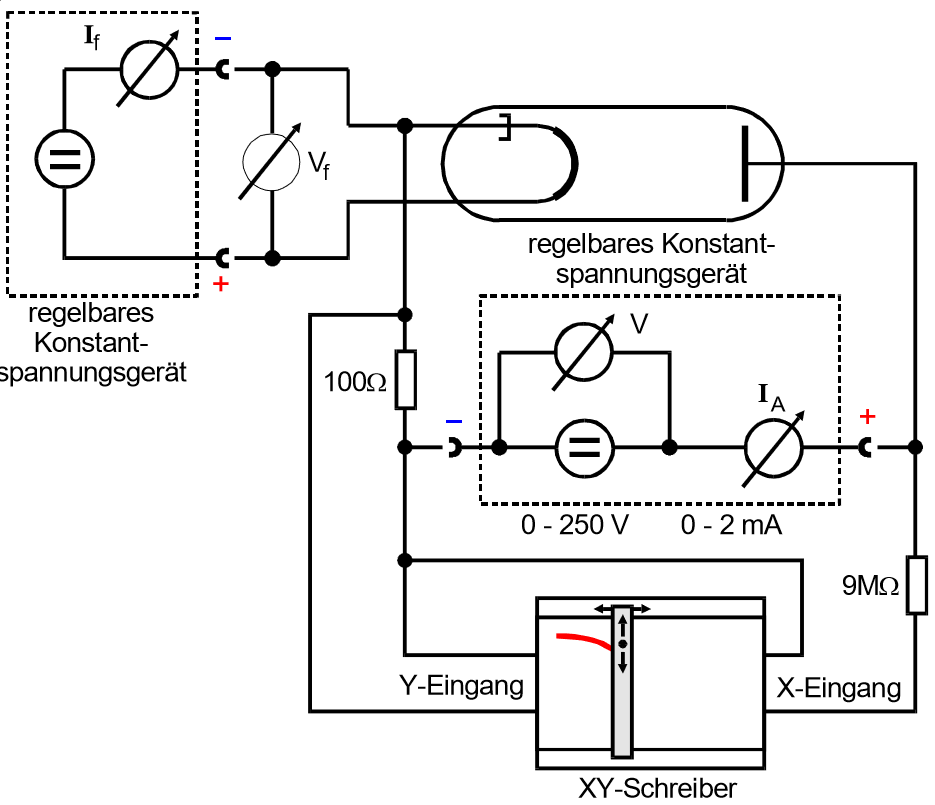
\includegraphics[width=10 cm, height= 7.5cm]{content/Aufbau1.png}
  \caption{Schaltdarstellung zur Aufnahme der Kennlinie \cite{1}.}
  \label{abb:4}
\end{figure}
Es steht kein XY-Schreiber zur Verfügung, also werden die Messwerte an ein separates Voltmeter-
bzw. Strommessgerät abgelesen und notiert.
Es werden fünf Kennlinie mit unterschiedlichen Heizströme gemessen, um den Sättigungsstrom
$I_s$ abzulesen zu können.
Um die Gültigkeit der Gleichung \ref{eq:2} zu überprüfen, wird ein maximaler Heizstrom
angeschlossen. Für diese Diode liegt dieser bei $\SI{2.4}{\ampere}$.
Aus dem Heizstromkreis wird noch die Temperatur der Kathode bestimmt.
Ebenso wird aus den fünf verschiedenen Kennlinie die Austrittsarbeit der Elektronen bestimmen.
Das verwendet Metall ist hier Wolfram.\\
Außerdem wird das Anlaufstromgebiet gemessen. Dazu wird die Schaltung in Abbildung \ref{abb:5}
verwendet.
\begin{figure}[H]
  \centering
  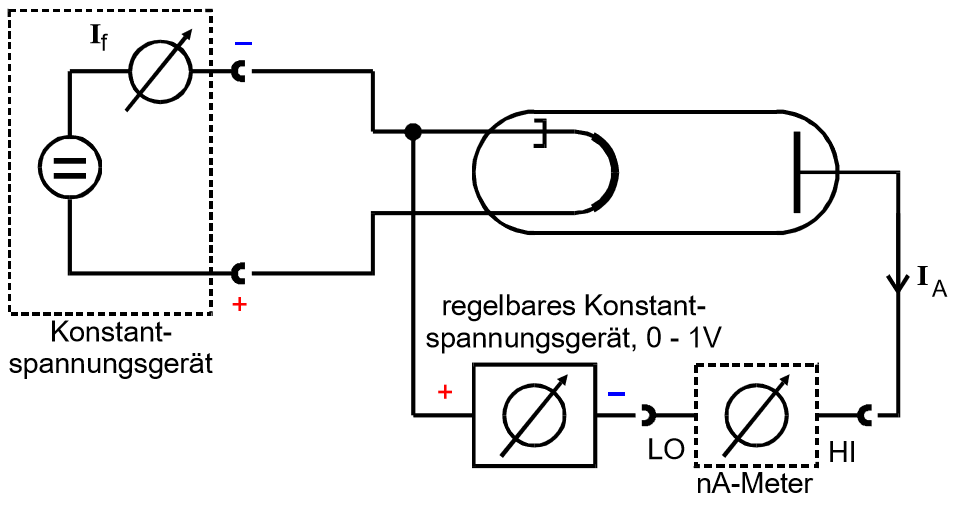
\includegraphics[width=10 cm, height= 7.5cm]{content/Aufbau2.png}
  \caption{Schaltdarstellung zur Aufnahme des Anlaufstromgebietes \cite{1}.}
  \label{abb:5}
\end{figure}
Da der Strom ziemlich klein ist, ist es wichtig, dass keine Störfaktoren wie Berührung des
Verbindungskabels gibt.
